\section{Properties of the Wigner distribution}
\label{app:wigner}

Here we present important properties of the Wigner distribution that are used throughout the paper.

\begin{proposition}\label{thm:wstate}
    The Wigner distribution of a state $\rho$ is
    \begin{enumerate}
        \item\label{en:w1} Real valued: $\W{\rho} \in \mathbb{R}^{d^2}$;
        \item\label{en:w2} Normalised: $\sum_{\bmz \in \pd} \W[\bmz]{\rho}=1$;
        \item\label{en:w3} Bounded: $\abs{\W[\bmx]{\rho}} \leq \frac{1}{d}$.
        \item\label{en:w4} Additive under mixing:
        
        $\W[\bmx]{\sum_i p_i \rho_i} = \sum\limits_i p_i \W[\bmx]{\rho_i}$;
        \item\label{en:w5} Multiplicative under tensor products: 
        
        $\W[\bmx_A \oplus \bmx_B]{\rho_A \otimes \rho_B} = \W[\bmx_A]{\rho_A}\W[\bmx_B]{\rho_B}$.
	\end{enumerate}
\end{proposition}
A distribution satisfying the first three properties does not necessarily correspond to a positive semi-definite state.

\begin{proposition}
    \label{thm:wchannel}
    The Wigner distribution of a $\cptp$ operation $\E: \cal{B}(\hd[d_A]) \mapsto \cal{B}(\hd[d_B])$ is:
    \begin{enumerate}
        \item\label{en:wo1} Real-valued: $\W[\bmy|\bmx]{\E} \in \mathbb{R}$;
        \item\label{en:wo2} Normalised: $\sum_{\bmz \in \pd[d_B]} \W[\bmz|\bmx]{\E} = 1$ for any $\bmx \in \pd[d_A]$;
        \item\label{en:wo3} Bounded: $\abs{\W[\bmy|\bmx]{\E}} \leq \frac{d_A}{d_B}$;
	    \item\label{en:wo4} \nick{Transitive}: $\W[\bmy]{\E(\rho)} = \sum_{\bmz \in \pd[d_A]} \W[\bmy|\bmz]{\E} \W[\bmz]{\rho}$ for any $\bmy \in \pd[d_B]$.
    \end{enumerate}
\end{proposition}
If $d_A = d_B$, and in particular if operation $\E$ maps a Hilbert space onto itself, then the stochasticity condition $\abs{\W[\bmy|\bmx]{\E}} \leq 1$ is satisfied.

%%%

\section{Properties of majorization}
\label{app:major}

\subsection{Equivalent conditions for majorization}

Any $\bmd$-majorization problem can be rephrased as a majorization problem in a higher dimensional space due to the embedding map.
\begin{definition}
    The embedding map $\Gamma_{\bmd}:\mathbb{R}^n \mapsto \mathbb{R}^D, D = \sum\limits_{i=1}^n d_i$ is the function
    \begin{equation}
        \Gamma_{\bmd}(\bmz) = \bigoplus_{i=1}^n z_i\  \frac{1}{d_i}\bm{1},
    \end{equation}
    where $\bm{1}/d_i$ is the $d_i$-dimensional uniform distribution.
    The left inverse $\Gamma_{\bmd}^{-1}: \mathbb{R}^D \mapsto \mathbb{R}^n$ is defined to sum up the elements in each block of $\Gamma_{\bmd}(\bmz)$, so that
    \begin{equation}
        \Gamma_{\bmd}^{-1}(\oplus_{i=1}^n z_i \bm{1}/d_i) = \bmz.
    \end{equation}
    This is not a right inverse, because $\Gamma_{\bmd}$ is not surjective.
\end{definition}
The direct sum simply amounts to listing the uniform distributions one after the other.
The embedding map maps the Gibbs distribution to the uniform distribution, $\Gamma_{\bmd}(\bmd) = \bm{1}/D$.
Then, a non-increasing ordering $\Gamma_{\bmd}(\bmz)^\downarrow$ in the new space, corresponds to the so-called ``$\beta$-ordering'' of the original vector denoted by the permutation $\pi$ mapping $(z_i/d_i) \mapsto (z_i/d_i)^\downarrow$ for all $i=1,\dots,n$.
Intuitively, $\beta$-ordering tends to simply non-increasing ordering as $\beta$ tends to 0.
This ordering naturally leads to a generalised notion of the Lorenz curve. 

\begin{theorem}
Given $\bmx, \bmy, \bmd \in \mathbb{R}^n$, such that the components of $\bmd$ are positive, the following statements are equivalent:
 \begin{enumerate}%[\rm{(TM1)}]
	\item $\bmx \prec_{\bmd} \bmy$;
	\item $\Gamma_{\bmd}({\bmx}) \prec \Gamma_{\bmd}({\bmy})$;
	\item\label{en:tm3} $\sum\limits_{i=1}^n \abs{x_i - t d_i} \leq \sum\limits_{i=1}^n \abs{y_i - t d_i}$ for all $t \in \mathbb{R}$;
	\item $\sum\limits_{i=1}^n (x_i - t d_i)^+ \leq \sum\limits_{i=1}^n (y_i - t d_i)^+$ for all $t \in \mathbb{R}$ and $\sum\limits_{i=1}^n x_i = \sum\limits_{i=1}^n y_i$;
	\item $\forall k, L_{\bmx|\bmd}(k) \leq L_{\bmy|\bmd}(k)$ and $L_{\bmx|\bmd}(k=n) = L_{\bmy|\bmd}(k=n)$.
 \end{enumerate}
\end{theorem}
\begin{proof}
    \begin{enumerate}
        \item[1$\leftrightarrow2$]
        Suppose now there exists a stochastic $S$ such that $\bmx = S\bmy$ with $\bmd = S\bmd$ and let $B = \Gamma_{\bmd} \circ S \circ \Gamma_{\bmd}^{-1}$.
        $B$ is a $D$-dimensional bistochastic matrix, since composition of stochastic matrices is stochastic and $(\Gamma_{\bmd} \circ S \circ \Gamma_{\bmd}^{-1}) (\frac{1}{D}\bm{1}) = (\Gamma_{\bmd} \circ S) (\bm{d}) = \Gamma_{\bmd}(\bm{d}) = \frac{1}{D}\bm{1}$. Then, $B$ maps $\Gamma_{\bmd}({\bmy})$ to $\Gamma_{\bmd}({\bmx})$.
        Conversely, given $B$, let $S = \Gamma_{\bmd}^{-1} \circ B \circ \Gamma_{\bmd}$.
        Similarly, $S$ is the stochastic matrix that preserves $\bmd$ and maps $\bmy$ to $\bmx$.
        \item[$2\leftrightarrow3$]\hspace{-5pt}, $2\leftrightarrow4$, $2\leftrightarrow5$ These three statement are equivalent to \nick{blah} respectively for the embedded vectors $\Gamma_{\bmd}({\bmx}), \Gamma_{\bmd}({\bmy})$.
        This is clear by rewriting
        \begin{align}
            \sum\limits_{i=1}^n \abs{x_i - t d_i} &= \sum\limits_{i=1}^n d_i \abs{\frac{x_i}{d_i} - t} = \sum\limits_{i=1}^D \abs{\Gamma_{\bmd}(\bmx)_i - t}, \\
            \sum\limits_{i=1}^n (x_i - t d_i)^+ &= \sum\limits_{i=1}^D (\Gamma_{\bmd}(\bmx)_i - t)^+, \\
            L_{\bmx|\bmd}(k) &= L_{\Gamma_{\bmd}(\bmx)}(k'), \\
            \text{with}\ k&=1,\dots,n\ \text{and}\ k'=1,\dots,D \nonumber
        \end{align} 
        and similarly for the right hand side.
    \end{enumerate}
\end{proof}

The Lorenz curve can be explicitly expressed as
    \begin{equation}
		\lc{\rho}{\sigma}(x) = (\bmu^\downarrow)_i x + \lc{\rho}{\sigma}(i) - (\bmu^\downarrow)_i x_i,\ x \in (x_{i-1}, x_i],
	\end{equation}
	for all $i=1,\dots,d$ with $x_0 \coloneqq 0$.

\subsection{Mana properties}
Mana monotonicity in any $\sigma$--fragment can be directly seen due to statement~\ref{en:tm3} in~\cref{thm:dmajor} for $t=0$.
Furthermore, mana is additive due to the multiplicative property~\ref{en:w4} of~\cref{thm:wstate}.

%%%

\section{Properties of $\sigma$-fragments}
\label{app:frag}

\begin{theorem}\label{thm:frag}
    Let $\R = (\O, \F)$ be a magic theory. 
    The following statements hold:
    \begin{enumerate}
        \item No $\sigma$-fragment is empty.
        \item If a free operation leaves two states invariant, then it also leaves their mixtures invariant, 
        \begin{equation}
            \O_{\sigma} \cap \O_{\sigma'} \subseteq \O_{p\sigma + (1-p)\sigma'}\ \text{for all}\ p \in [0,1].
        \end{equation}
        \item Let $\E$ be a $\cptp$ operation with Wigner distribution $\W{\E}$.
        For $\R = \Rmax$ $\E \in \O_\sigma$ iff $\W{\E} \in \stochw$.
    \end{enumerate}
\end{theorem}
\begin{proof}$ $\\

    \begin{enumerate}
    \item The identity channel $1_{\rm{C}}: \D \mapsto \D$ belongs to every $\sigma$-fragment, as $1_{\rm{C}} \in \O$ and $1_{\rm{C}}\sigma = \sigma$ for all $\sigma \in \F$.
    
    \item Let $\E \in \O_{\sigma} \cap \O_{\sigma'}$.
    Then $\E \in \cptp$ and corresponds to stochastic Wigner distribution $\W{\E}$ such that $\W{\E} \W{\sigma} = \W{\sigma}$ and $\W{\E} \W{\sigma'} = \W{\sigma'}$.
    Then, $\W{\E} \W{p\sigma + (1-p)\sigma'} = \W{p\sigma + (1-p)\sigma'}$ for any $p \in [0,1]$ due to the additive property~\ref{en:w4} of the Wigner distribution, implying that state $p\sigma + (1-p)\sigma'$ is also left invariant by $\E$.
    
    \item Let $\O_\sigma' \coloneqq \{ \E \in \cptp: \W{\E} \in \stochw \}$ be the described set of operations.
    
    Suppose $\E$ is in $\O_\sigma$, then $\E \in \cptp$ and $\W{\E} \in \stochw$ due to property~\ref{en:wo4} of~\cref{thm:wchannel}, hence $\O_\sigma \subseteq \O_\sigma'$.
    
    Conversely, suppose $\E \in \cptp$ with $\W{\E} \in \stochw$. 
    Then, $\W[\bmy|\bmx]{\E} \geq 0$ for all $\bmx, \bmy$, hence $\E \in \O$.
    Furthermore, $\W{\E} \W{\sigma} = \W{\sigma}$ implies $\E(\sigma) = \sigma$ using~\cref{eq:woperation} defined for any $\cptp$ operation $\E$.
    Hence, $\O_\sigma' \subseteq \O_\sigma$.
    \end{enumerate}
\end{proof}

Any free state $\sigma \in \cal{B}(\hd)$ corresponds to a $d^2$-dimensional probability distribution $\W{\sigma}$ and any free operation $\E: \cal{B}(\hd) \mapsto \cal{B}(\hd)$ corresponds to a $d^2 \times d^2$ stochastic matrix (or conditional probability distribution) $\W{\E}$.
Note that these mappings are one-to-one due to the orthogonality of the phase-point operators as an operator basis.

\emph{Remark 1.} Note that free states $\F$ are mapped onto a \emph{strict subset} of the set of probability distributions.
As a counterexample, the sharp $d^2$-dimensional probability distribution $(1, 0, \dots, 0)$ does not correspond to any qudit Wigner distribution because of the boundedness condition~\ref{en:w3} in~\cref{thm:wstate}.

\emph{Remark 2.} Similarly, not all stochastic matrices correspond to completely positive operations.

As an example, consider the permutation matrix
\begin{equation}
    \Pi_X = \begin{psmallmatrix}
        0 & 1 & 0 & 0 & 0 \\
        0 & 0 & 0 & 0 & 1 \\
        0 & 0 & 0 & 1 & 0 \\
        1 & 0 & 0 & 0 & 0 \\
        0 & 0 & 1 & 0 & 0
    \end{psmallmatrix} \otimes \begin{psmallmatrix}
        0 & 0 & 1 & 0 & 0 \\
        0 & 0 & 0 & 0 & 1 \\
        0 & 0 & 0 & 1 & 0 \\
        1 & 0 & 0 & 0 & 0 \\
        0 & 1 & 0 & 0 & 0    
    \end{psmallmatrix} \in \stochw,\ d=5.
\end{equation}
It preserves the uniform distribution $\W{\frac{1}{5}\id}{}$, but it does not correspond to any $\cpos$ operation, hence any $\E \in \O$ due to~\cref{thm:frag}.

\section{Area monotone}
\label{app:areamono}

\begin{figure}[t]%
    \centering
    \subfigure[][]{%
    \label{fig:test1}%
    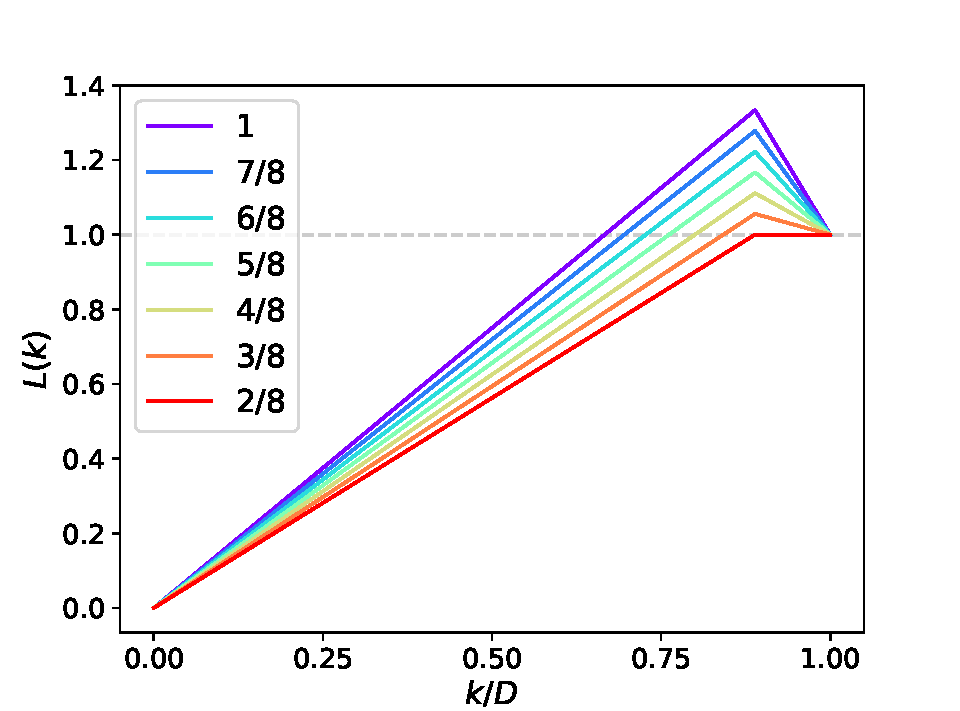
\includegraphics[height=3cm]{figs/negmasking_rho_strange_lc.pdf}
    %\caption{Maximally mixed state $\frac{1}{3}\id$}%
    }\hspace{8pt}%
    \subfigure[][]{%
    \label{fig:test2}%
    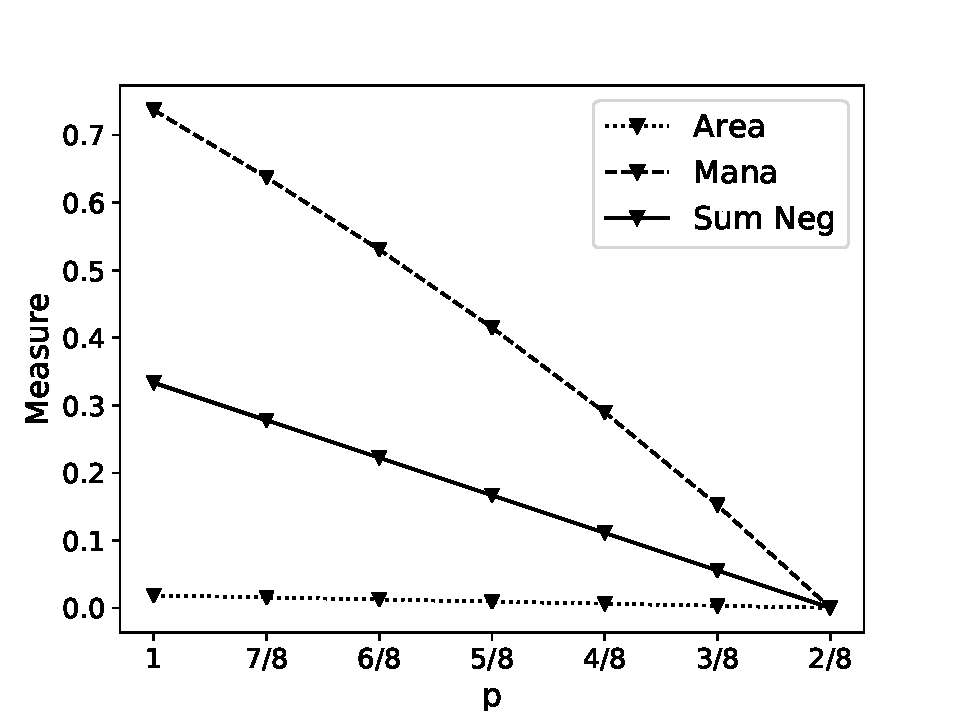
\includegraphics[height=3cm]{figs/negmasking_rho_strange_meas.pdf}
    %\caption{Zero state $\ketbra{0}{0}$}%
    }
    \caption{\subref{fig:test1} Lorenz curve of $p\ketbra{\rm{S}} + (1-p) \frac{1}{d}\id$ for $p$ given in the legend.\subref{fig:test2} Different measures for the states on the left. \\
    \nick{can replace~\cref{fig:lctoy} with a more informative version of this figure}
    }%
    \label{fig:test}
\end{figure}

Let $L_{>1}$ be the set of points on the Lorenz curve $\lc{\rho}{\sigma}(k)$ that lie above $1$ of state $\rho$ in the $\sigma$--fragment. 
If $\rho$ is a free state, $L_{>1}$ is empty and $\A_\sigma(\rho) = 0$. 
Otherwise, $\A_\sigma(\rho) > 0$ and it can be calculated exactly using the trapezium rule or the shoelace formula. 
Let $k$ be the index of the first point $\left(x_k, \lc{\rho}{\sigma}(k)\right)$ lying above $1$. 
Then $L_\rho(k)$ crosses $1$ at
\begin{equation}
	x_{\rm{int}} = x_k - \frac{x_k - x_{k-1}}{\lc{\rho}{\sigma}(k) - \lc{\rho}{\sigma}(k-1)}\lc{\rho}{\sigma}(k),\vspace{10pt}
\end{equation}
as well as at $\left(x_d, \lc{\rho}{\sigma}(d)\right) = (1,1)$

Now we can define
\begin{equation}
L_{>1}^+ = \{ (x_i, y_i) \}_{0 \leq i \leq n}
\end{equation}
such that it contains the initial point of intersection $(x_0, y_0) \equiv (x_{n+1}, y_{n+1}) \coloneqq (x_{\rm{int}}, 1)$, all points $(x_i, y_i)$, labelled by $i=1,\dots,n-1$ that lie above $y=1$ contained in $L_{>1}$ and finally the second point of intersection $(x_n, y_n) = (1,1)$.
Then, 
\begin{equation}
	\A_\sigma(\rho) = \frac{1}{2} \sum\limits_{i=0}^n (x_{i+1} y_i - x_i y_{i+1}).
\end{equation}

\section{Technical derivations for standard Lorenz curves}
\label{app:lcsu_technical}

\subsubsection{Binomial distributions and error bounds}
Consider an experiment consisting of $n$ trials of throwing a $p$-coin, that is a coin with probability $p$ of landing on one side and $1-p$ of landing on the other.
This scenario describes the construction of an $n$-copy Strange state Wigner distribution from a single-copy as presented in~\cref{sec:lcsu}.
The experiment is described by binomial statistics and we write down the sum over an even number of successful trials $\Phi_+$ (over an odd number of successful trials $\Phi_-$),
\begin{align}	
	\Phi_+(m; n, p) &\coloneqq \sum\limits_{j=0}^{m/2} \binom{n}{2j} p^{2j} (1-p)^{n-2j}, \nonumber\\ 
	&\text{for even integers } m\in[0,n], \label{eq:fp} \\
	\Phi_-(m; n, p) &\coloneqq \sum\limits_{j=1}^{(m-1)/2} \binom{n}{2j+1} p^{2j+1} (1-p)^{n-(2j+1)}, \nonumber\\ 
	&\text{for odd integers } m\in[0,n]. \label{eq:fn2}
\end{align}
Note that index $m$ only takes even (odd) values when labelling $\Phi_+$ ($\Phi_-$).
$\Phi_+$ describes the elbow coordinates on the LHS of the curve maximum, including the maximum, while $\Phi_-$.

We define the classical relative entropy between a $p$-coin and a $q$-coin as
\begin{equation}\label{eq:ent_rel}
	\ent{p}{q} \coloneqq p \log{\frac{p}{q}} + (1-p) \log{\frac{1-p}{1-q}}.
\end{equation}
It satisfies the identity $\ent{p}{q} = \ent{1-p}{1-q}$.

The classical entropy of a $p$-coin is
\begin{equation}\label{eq:ent}
	S(p) \coloneqq -p\log{p} -(1-p)\log{(1-p)},
\end{equation}
which is symmetric, $S(p) = S(1-p)$.
%Let $c(m; n) \coloneqq [m(1-m/n)]^{-1/2},\ m\in [1, n-1]$.
A useful result is the entropic bound on a combination~\cite{cit:ash}.
\begin{lemma}\label{lem:comb_bounds}
	For all $m\in [1,n-1]$,
	\begin{align}
		&\left[ 8m\left(1-\frac{m}{n}\right) \right]^{-\frac{1}{2}} 2^{nS\left(\frac{m}{n}\right)} \leq \binom{n}{m} \leq \\
		&\left[ 2\pi m\left(1-\frac{m}{n}\right) \right]^{-\frac{1}{2}} 2^{nS\left(\frac{m}{n}\right)}.
	\end{align}
\end{lemma}
\begin{proof}
	For $m = 1,2, n-1, n-2$ check by direct calculation.	
	For all other cases, use Stirling's approximation.
\end{proof}

Bounds on the tails of a cumulative binomial distribution can be expressed in

and therefore we can use $\Phi_{\pm}$ to compactify statements that hold for both $\Phi_+, \Phi_-$.

\iffalse
The experiment is described by binomial statistics and we define the left tail of the cumulative binomial distribution,
\begin{equation}\label{eq:phil}
	\Phi_\ell(m; n, p) \coloneqq \sum\limits_{j=0}^m \binom{n}{j} p^j (1-p)^{n-j},
\end{equation}
where $m\in [0,n]$. 

The symmetry between the left tail of a $p$-coin distribution and the right tail of a $(1-p)$-coin distribution dictates that
\begin{align}\label{eq:phi_reverse}
	\Phi_\ell(m; n, p) + \Phi_\ell(n-m-1; n, 1-p) &= 1,\ m\in [0,n-1],
\end{align}
Entropic bounds on $\Phi_\ell$~\cite{cit:ash}.
\begin{lemma}\label{lem:phil_bounds}
	Given fixed $n>0$ and $p$, $\Phi_\ell$ satisfies the following bounds:
	\begin{align*}
		\begin{split}
		&\text{1. } \Phi_\ell(m; n, p) \geq \left[ 8m\left(1-\frac{m}{n}\right) \right]^{-\frac{1}{2}} 2^{-n\ents},\ m\in [1,n-1] \\
		&\text{2. } \Phi_\ell(m; n, p) \leq 2^{-n\ents},\ m\in [0,np] \\
		&\text{3. } \Phi_\ell(m; n, p) \leq 1 - \left[ 8(m+1)\left(1-\frac{m+1}{n}\right) \right]^{-\frac{1}{2}} 2^{-n\ent{\frac{m+1}{n}}{p}}, \\
		&\hspace{14pt} m\in [0,n-2]
		\end{split}
		\\
		&\text{4. } \Phi_\ell(m; n, p) \geq 1 - 2^{-n\ent{\frac{m+1}{n}}{p}},\ m\in [np+1,n-2]
	\end{align*}
\end{lemma}
\begin{proof}
	\nick{cite proof}
\end{proof}

In particular, we derive ``loose'' and ``strict'' bounds on $\Phi_{\pm}$.
\begin{lemma}\label{lem:bounds_loose}
	Given fixed $n>0$ and $p$, $\Phi$ satisfies the following bounds:
	\begin{align*}
		\begin{split}
		&\text{1. } \Phi_{\pm}(m; n, p) \geq \left[ 8m\left(1-\frac{m}{n}\right) \right]^{-\frac{1}{2}} 2^{-n\ents},\ m\in [1,n-1] \\
		&\text{2. } \Phi_{\pm}(m; n, p) \leq 2^{-n\ents},\ m\in [0,np] \\
		&\text{3. } \Phi_{\pm}(m; n, p) \leq 1 - \left[ 8(m+1)\left(1-\frac{m+1}{n}\right) \right]^{-\frac{1}{2}} 2^{-n\ent{\frac{m+1}{n}}{p}}, \\
		&\hspace{14pt} m\in [0,n-2]
		\end{split}
	\end{align*}
\end{lemma}
\begin{proof}
	\nick{paste proof}
\end{proof}
\begin{lemma}\label{lem:bounds_strict}
	Given fixed $n>0$ and $p$, $\Phi_+, \Phi_-$ satisfy the following bounds:
	\begin{align*}
		\begin{split}
		&\text{1. } \Phi_+(m; n, p) \geq \sum\limits_{j=0}^{m/2}\left[ 8(2j)\left(1-\frac{2j}{n}\right) \right]^{-\frac{1}{2}} 2^{-n\ent{\frac{2j}{n}}{p}}, \\
		&\hspace{14pt} \text{for all even } m\in [2,n] \\
		&\text{2. } \Phi_+(m; n, p) \leq \sum\limits_{j=0}^{m/2}\left[ 2\pi(2j)\left(1-\frac{2j}{n}\right) \right]^{-\frac{1}{2}} 2^{-n\ent{\frac{2j}{n}}{p}}, \\
		&\hspace{14pt} \text{for all even } m\in [2,n] \\
		&\text{3. } \Phi_-(m; n, p) \geq \sum\limits_{j=1}^{(m-1)/2}\left[ 8(2j+1)\left(1-\frac{2j+1}{n}\right) \right]^{-\frac{1}{2}} \times \\
		&\hspace{14pt} \times 2^{-n\ent{\frac{2j+1}{n}}{p}},\ \text{for all odd } m\in [1,n] \\
		&\text{4. } \Phi_-(m; n, p) \leq \sum\limits_{j=1}^{(m-1)/2}\left[ 2\pi(2j+1)\left(1-\frac{2j+1}{n}\right) \right]^{-\frac{1}{2}} \times \\
		&\hspace{14pt} \times 2^{-n\ent{\frac{2j+1}{n}}{p}},\ \text{for all odd } m\in [1,n]
		\end{split}
	\end{align*}
\end{lemma}
\begin{proof}
	\nick{paste proof}
\end{proof}
\fi

They are depicted in~\cref{fig:noisys}.
\begin{figure}[t]
    \centering
    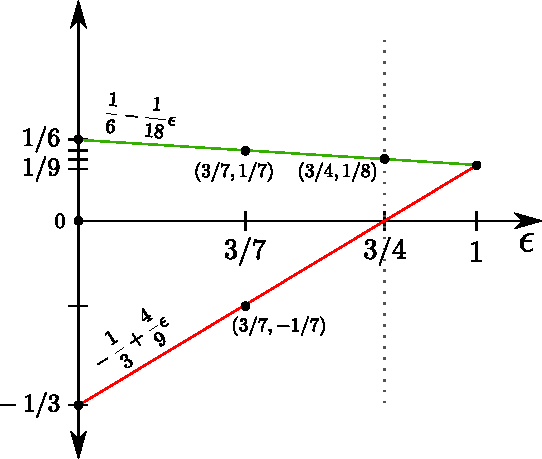
\includegraphics[scale=0.7]{figs/noisys.pdf}
    \caption{\textbf{Wigner components of the noisy Strange state.} 
    In the interval $0 \leq \epsilon < 3/7$, the negative component is larger than the positive components.
    At $\epsilon = 3/7$ the Wigner distribution is $(-\frac{1}{7},\frac{1}{7},\dots,\frac{1}{7})$.
    In the interval $3/7 < \epsilon < 3/4$, the positive components are larger than the negative component.
    In the interval $3/4 \leq \epsilon \leq 1$, there is no negativity.
    }
    \label{fig:noisys}
\end{figure}
The $n+1$ distinct Wigner components ($w_j$) of $\noisysn$ along with their multiplicities ($m_j$) are given in~\cref{tab:lcsu_w}.
\begin{table}[b]                           
 \centering
 \begin{tabular}{c|c|c|c}
 $\epsilon$ & $j$ & $\left[0, \frac{n}{2}\right]$ & $\left[\frac{n}{2} + 1, n \right]$ \\ [0.5ex] 
 \hline
  & $w_{j}$ & $w_+^{2j}w_-^{n-2j}$ & $w_+^{n-2j}w_-^{2j}$  \\
  $0\leq \epsilon < \frac{3}{7}$ & & & \\
  & $m_{j}$ & $8^{2j}\binom{n}{2j}$ & $8^{n-2j}\binom{n}{2j}$ \\
 \hline
  & $w_{j}$ & $w_+^{n-2j}w_-^{2j}$ & $w_+^{2j}w_-^{n-2j}$  \\
  $\frac{3}{7} \leq \epsilon < \frac{3}{4} $ & & & \\
  & $m_{j}$ & $8^{n-2j}\binom{n}{2j}$ & $8^{2j}\binom{n}{2j}$
\end{tabular}
 \caption{Wigner components of $\noisysn$. The multiplication $2j$ is modulo $(n+1)$.}
 \label{tab:lcsu_w}
\end{table}



To get the Lorenz curve, we need to sum up the Wigner components in decreasing order and the order depends on the noise level $\epsilon$, so we define probabilities associated with the $x$-coordinate ($p_x$) and the vertical coordinate ($p_L$) of the Lorenz curve accordingly,
\begin{equation}
	(p_x, p_L) \equiv \big( p_x(\epsilon), p_L(\epsilon) \big) = 
	\begin{cases}
		\left( \frac{8}{9}, \frac{12-4\epsilon}{15-8\epsilon} \right),\ & 0\leq \epsilon < \frac{3}{7} \\
		\left( \frac{1}{9}, \frac{3-4\epsilon}{15-8\epsilon} \right),\ & \frac{3}{7}\leq \epsilon < \frac{3}{4} \\
	\end{cases}	
\end{equation}

We are now in a position to express Lorenz curve coordinates in terms of phi distributions,
\begin{equation}\label{eq:x_coord_elb}
	x_k(n, \epsilon) = 
	\begin{cases}
		\Phi_+(k;n,p_x),\\
		\hspace{20pt} k\in[0,n]\ \text{and }k\text{ even}, \\
		x_{k_\star} + \Phi_-(k;n,1-p_x),\\
		\hspace{20pt} k\in[0,n]\ \text{and }k\text{ odd}, \\
	\end{cases}	
\end{equation}
and
\begin{equation}\label{eq:lc_coord_elb}
	L_k(n, \epsilon) = 
	\begin{cases}
		\left( \frac{5}{3} - \frac{8}{9}\epsilon\ \right)^n \Phi_+(k;n,p_L),\\
		\hspace{20pt} k\in[0,n]\ \text{and }k\text{ even}, \\
		L_{k_\star} - \left( \frac{5}{3} - \frac{8}{9}\epsilon\ \right)^n\Phi_-(k;n,1-p_L),\\
		\hspace{20pt} k\in[0,n]\ \text{and }k\text{ odd}. \\
	\end{cases}	
\end{equation}

Finally, the $m$-th elbow is located at
\begin{equation}\label{eq:lcsu_elbows}
	\left(x_m, \lc{\noisysn}{\frac{1}{d}\id}(x_m) \right) = \Big( x_{2m}(n, \epsilon), L_{2m}(n, \epsilon) \Big),
\end{equation}
where $2m$ is considered \hspace{-7pt}$\mod{(n+1)}$.

We can therefore use~\cref{lem:bounds_loose,lem:bounds_strict} to bound the standard Lorenz curves.
\begin{figure}[b]
    \centering
    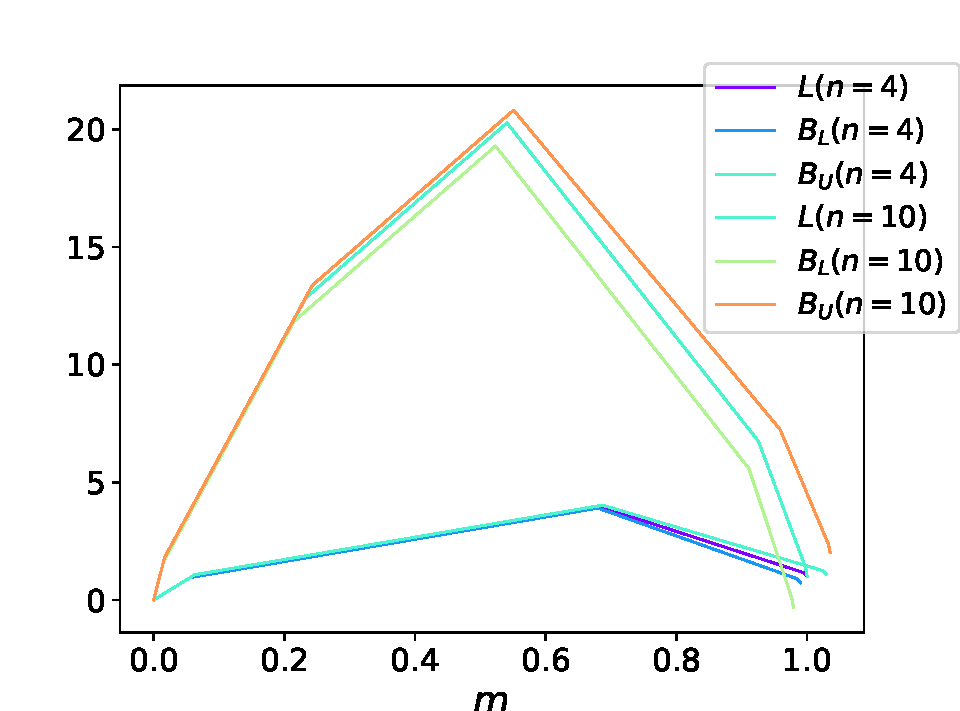
\includegraphics[scale=0.4]{figs/lc_bounds.pdf}
    \caption{\textbf{Lorenz curves and bounding curves.} 
    The figure explores the distillation process of a 10-copy $0.25$-noisy Strange state to a 4-copy $0.05$-noisy Strange state in the unital fragment.
    Clearly, by looking at the Lorenz curves, the distillation process is possible.
    However the bounding curves, derived in~\cref{lem:bounds_strict}, intersect at the end, suggesting that the process is not necessarily possible.
    }
    \label{fig:lc_bounds}
\end{figure}


Assume: 
\begin{itemize}
    \item $n$ is even [ensures Lorenz curve coordinates can be expressed in terms of $\Phi_{\pm}$ distributions];
    \item $0 \leq \epsilon \leq \frac{3}{7}$ [ensures closed-form expressions for Lorenz curve coordinates];
\end{itemize}
There are $\frac{n}{2}+1$ distinct non-negative components in the Wigner distribution $\W{\noisysn}$.\\

We can rewrite the non-negative part of the Wigner distribution $\W{\noisysn}$ in a compact form, by simply listing the distinct Wigner components $w(k; n, \epsilon)$ along with their multiplicities $m(k; n)$:
\begin{align}
    &{\W{\noisysn}} = \\ 
    &\big\{\left( m_k, w_k \right)\big\}_{k=0,\dots,n/2} = \nonumber\\ 
    &\big\{\left( m(k; n), w(k; n, \epsilon) \right)\big\}_{k=0,\dots,n/2} = \nonumber\\
    &\left\{ \left( 8^{2k}\binom{n}{2k}, \left( \frac{1}{6} - \frac{1}{18}\epsilon \right)^{2k}\left( -\frac{1}{3} + \frac{4}{9}\epsilon \right)^{n-2k} \right) \right\}_{k=0,\dots,n/2}. \nonumber
\end{align}

The expressions for the Lorenz curve elbows in the unital fragment are then known:
\begin{align}
    &{\rm{L}_{\noisysn}} = \\
    &\big\{\left( x_k, L_k \right)\big\}_{k=0,\dots,n/2} = \nonumber\\
    &\big\{\left( x(k; n), L(k; n, \epsilon) \right)\big\}_{k=0,\dots,n/2} = \nonumber\\
    &\left\{ \left( \frac{1}{9^n}\sum\limits_{j=0}^k m_j, \sum\limits_{j=0}^k m_j w_j \right) \right\}_{k=0,\dots,n/2} = \nonumber\\
    &\left\{ \left( \Phi_+\left(2k;n,\frac{8}{9}\right), \left( \frac{5}{3} - \frac{8}{9}\epsilon\ \right)^n \Phi_+\left(2k;n,4\frac{3-\epsilon}{15-8\epsilon}\right) \right) \right\}_{k=0,\dots,n/2}. \nonumber
\end{align}
We include the origin in the Lorenz curve as it does not arise from the above expressions, denoting it by $(x_{-1}, L_{-1}) \coloneqq (0,0)$.

We can get explicit expressions for all $\frac{1}{2}(7^n + 9^n)$ points of the Lorenz curve, using a two-index parameterisation:
\begin{align}
    x_{k,\alpha} &= \left( 1-\frac{\alpha}{m_k} \right) x_{k-1} + \frac{\alpha}{m_k} x_k \label{eq:x}\\
    L_{k,\alpha} &= \left( 1-\frac{\alpha}{m_k} \right) L_{k-1} + \frac{\alpha}{m_k} L_k \label{eq:l}\\
    &\text{for } k=0,\dots,\frac{n}{2} \text{ and } \alpha = 1,\dots,m_k. \nonumber
\end{align}

As a simple example, we plot the Lorenz curve of state $\noisys(0)\too{2}$,
\begin{figure}[h]
    \centering
    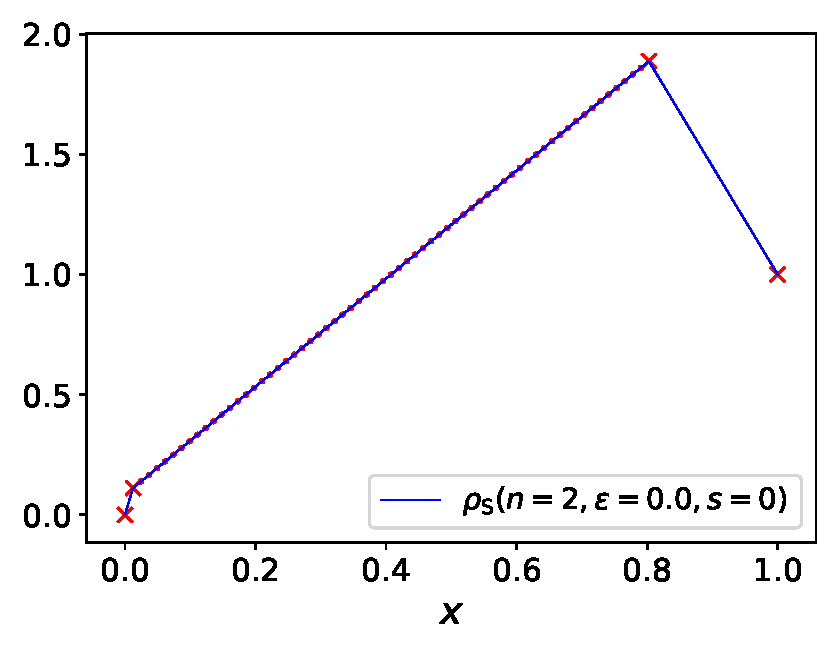
\includegraphics[scale=0.6]{figs/lcpoints.pdf}
    \caption{\textbf{All points on the Lorenz curve are uniformly distributed.}
    \cref{eq:x,eq:l}) capture the coordinates of all points up to the maximum.
    }
    \label{fig:lc}
\end{figure}

Consider now the state 
\begin{equation}
    \noisys(r, \epsilon, s) = \noisys(\epsilon)\too{r} \otimes \left( \frac{1}{3}\id \right)\too{s}.
\end{equation}

Tensoring with the maximally mixed state keeps the Lorenz curve unchanged, but increases the resolution of (the uniformly distributed) points.
The new point coordinates are given by:
\begin{align}
    x_{k,\alpha, \beta} &= \left( 1-p_{k,\alpha, \beta}\right) x_{k-1} + p_{k,\alpha, \beta} x_k \label{eq:lcsu_xcoord}\\
    L_{k,\alpha, \beta} &= \left( 1-p_{k,\alpha, \beta} \right) L_{k-1} + p_{k,\alpha, \beta} L_k, \label{eq:lcsu_lcoord}\\
    &\text{where } p(k, \alpha, \beta) = \frac{(\alpha-1)9^s + \beta}{9^s m_k} \\
    &\text{for } k=0,\dots,\frac{r}{2},\ \alpha = 1,\dots,m_k \text{ and } \beta = 1,\dots,9^s. \nonumber
\end{align}

We can unify the indices, by introducing a single index
\begin{equation}
    i(k,\alpha,\beta) \coloneqq \beta + \left[ (\alpha-1) + \sum_{j=0}^{k-1} 8^{2j}\binom{r}{2j} \right]9^s,
\end{equation}
so that $i=1,2,\dots, \frac{1}{2}9^s(7^{r} + 9^{r})$.
The $\frac{r}{2}$ elbows correspond to 
\begin{equation}
	i(k, \alpha, \beta) = i(\kappa, m_{\kappa}, 9^s) \equiv \sum_{j=0}^{\kappa} m_j,\ \kappa = 0,\dots,\frac{r}{2}.
\end{equation}
This index function is bijective, i.e.
\begin{equation}
	(k, \alpha, \beta) = (k', \alpha', \beta') \Leftrightarrow i(k, \alpha, \beta) = i(k', \alpha', \beta').
\end{equation}





